\chapter{Functions of Several variables}
\begin{thm}[23][Bananach's Fixed Point Theorem/Contraction Mapping Theorem]
	Let $(X,d)$ be a complete metric space. Suppose $\exists{c < 1} \text{ such that } $ the map $\phi:X\to X$ obeys $d(\phi(x),\phi(y))\le c d(x,y)$ for all $x,y \in X$ ($\phi$ is a \textit{ contraction }).
	Then $\exists{!} x \in X$ such that $\phi(x) = x$.
	\begin{proof}
		\begin{description}
			\item[Uniqueness:]
			      If $\phi(x)=x$ and $\phi(y)=y$, then $d(x,y)=d(\phi(x),\phi(y))\le c d(x,y)$, so $d(x,y)=0$ and $x=y$.
			\item[Existence:]
			      Given $x_{0} \in X$, let $x_{1}=\phi(x_{0}),x_{2}=\phi(x_{1})=(\phi \circ \phi)(x_{0})$, $x_{n+1}=\phi(x_n)=\underbrace{(\phi \circ \phi)}_{n+1}(x_{0})$.
			      Then $d(x_{n+1},x_n)=d(\phi(x_n), \phi(x_{n-1}))\le c d(x_n,x_{n-1})$, so by induction, $d(x_{n+1},x_n)\le c^{n}d(x_{1},x_{0})$ and hence for $n>m$,
			      \[
				      d(x_n,x_m)\le \sum_{i=m+1}^{n}{d(x_i,x_{i-1})}\le \sum_{i=m+1}^{n}{c^{i-1}d(x_{1},x_{0})} \le \sum_{i=m+1}^{\infty}{c^{i-1}d(x_{1},x_{0})}=\frac{c^{m}}{1-c} d(x_{1},x_{0}).\]
			      Hence, $\{x_n\}$ is a Cauchy sequence. As $X$ is assumed to be complete, $\exists x \in X$ such that $x_n \to x$. Since $\phi$ is continuous $\phi(x)=\lim_{n\to \infty}{\phi(x_n)}=\lim_{n\to \infty}{x_{n+1}}=x$.
		\end{description}

	\end{proof}
	\begin{remark}
		\begin{enumerate}
			\item $\phi$ is uniformly continuous ( take $\delta=\epsilon$ ).
			\item The proof gives an exponentially convergent algorithm to find the fixed point.
			\item Visualization of the algorithm used in the proof:\\
			      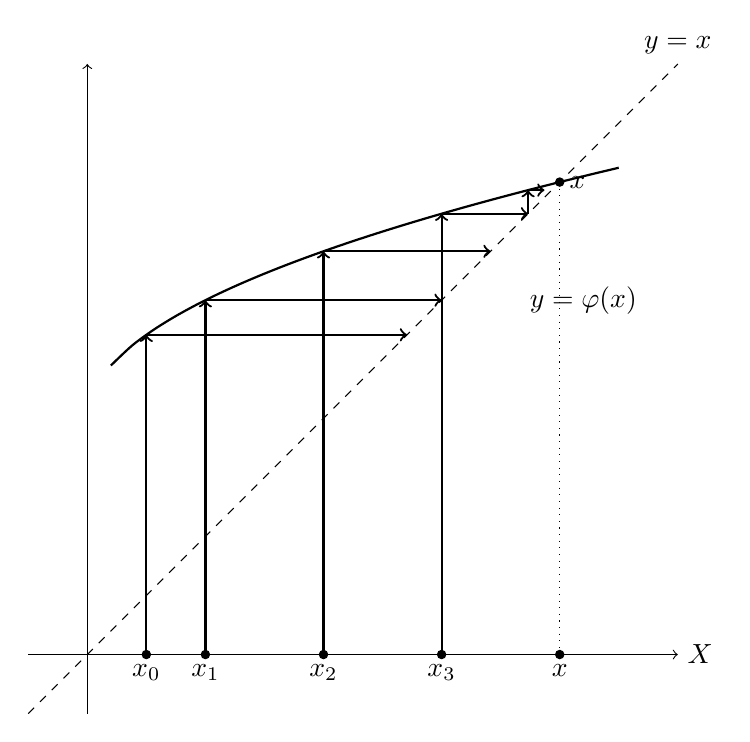
\begin{tikzpicture}[scale=1.5]
				      % Axes
				      \draw[->] (-0.5,0) -- (5,0) node[right] {$X$};
				      \draw[->] (0,-0.5) -- (0,5) node[above] {};

				      % y = x line
				      \draw[dashed] (-0.5,-0.5) -- (5,5) node[above] {$y = x$};

				      % Curve for y = \varphi(x)
				      \draw[thick, domain=0.2:4.5, smooth, variable=\x] plot ({\x},{sqrt(\x)+2});
				      \node at (4.2,3) {$y = \varphi(x)$};

				      % Points x0, x1, x2, x3, etc.
				      \foreach \x/\y/\name in {
				      0.5/{sqrt(0.5)+2}/x_0,
				      1/{sqrt(1)+2}/x_1,
				      2/{sqrt(2)+2}/x_2,
				      3/{sqrt(3)+2}/x_3
				      }{
				      \filldraw (\x,0) circle (1pt) node[below] {$\name$};
				      \draw[thick, ->] ({\x},0) -- ({\x},{\y});
				      \draw[thick, ->] ({\x},{\y}) -- ({\y},{\y});
				      }
				      % Converging to fixed point
				      \filldraw (4,{sqrt(4)+2}) circle (1pt);
				      \node[right] at (4,{sqrt(4)+2}) {$x$};

				      % Dotted line to x axis
				      \draw[thick, ->] ({sqrt(3)+2},{sqrt(3)+2}) -- ({sqrt(3)+2},{sqrt(sqrt(3)+2)+2});
				      \draw[thick, ->] ({sqrt(3)+2},{sqrt(sqrt(3)+2)+2}) -- ({sqrt(3.5)+2},{sqrt(sqrt(3)+2)+2});
				      % Labels
				      \node[below] at (4,0) {$x$};
				      \draw[dotted] (4,4) -- (4,0);
				      \filldraw (4,0) circle (1pt);

			      \end{tikzpicture}
		\end{enumerate}
		\item Reading assignment: Rudin's theorems 9.1-9.9.
	\end{remark}
\end{thm}

\section{Diffrentiation of functions of $f: \R^{n} \to \R^{m}$}

Recall for $n=m=1$,
\[
	f'(x)=\lim_{h\to \infty}{\frac{f(x+h)-f(x)}{h}}
	.\]

Equivalently, \[
	\lim_{h\to 0}{\left|\frac{f(x+h)-f(x)-f'(x)h}{h}\right|}=0
	.\]
This again is equivalent to
\[
	f(x+h)=f(x)+\underbrace{f'(x) h}_{\text{ best linear approximation to $f(x+h)-f(x)$ } }+\underbrace{r(h)}_{r(h)=o(h)}
	,\]
with $\lim_{h\to 0}{\frac{r(h)}{h}}=0$.


\begin{define}[11]
	Let $m,n \in \N$, $E \subset \R^{n}$ an open set, $f: E\to \R^{m}, x \in E$.
	Then $f$ is \textit{differentiable} at $x$ and $f'(x)=A$ if
	\[
		\lim_{h\to 0}{\frac{\|f(x+h)-f(x)-Ah\|}{\|h\|}}=0
		,\] where $A$ depends on $x$, $A \in L(\R^{n},\R^{m})$.
	Note $L(\R^{n},\R^{m})$ is the vector space of linear maps from $\R^{n}$ to $\R^{m}$.
	That is, if $f(x+h)=f(x)+Ah+r(h)$ with $\lim_{h\to 0}{\frac{\|r(h)\|}{\|h\|}}=0$.
\end{define}

\begin{notation}
	$r(h)=o(h)$ means $\lim_{h\to 0}{\frac{\|r(h)\|}{\|h\|}}=0$.
\end{notation}

\begin{thm}[12]
	$A$ in the definition of differentiability is unique if it exists.
	\begin{proof}
		Suppose
		\begin{flalign*}
			f(x+h) & =f(x)+A_{1}h + r_{1}(h) \\
			f(x+h) & =f(x)+A_{2}h + r_{2}(h) \\
			.\end{flalign*}
		with $r_{1}h=o(h), r_{2}h=o(h)$.
		Let $B=A_{1}-A_{2}$. Then $Bh=r_{2}(h)-r_{1}(h)$, so for a fixed $h\neq 0$ and $t>0$, \[
			\frac{\left|Bh\right|}{\left|h\right|}= \frac{\left|B(th)\right|}{\left|th\right|} \le \frac{\left|r_{2}(th)\right|}{th}+\frac{\left|r_{1}(th)\right|}{th}.\]
		$\frac{\left|Bh\right|}{\left|h\right|}$ is independent of $t$. Hence, $\frac{\left|Bh\right|}{\left|h\right|}\to 0$ as $h\to 0$ (think of $th=h'\to 0$).
		$Bh=0$ for all $h \in \R^{n}$; i.e., $B=0$; i.e., $A_{1}=A_{2}$.
	\end{proof}
	\begin{note}
		\begin{enumerate}
			\item If $f'(x)$ exists for all $x \in E$ then we can regard $f'$ as a function $f':E\to L(\R^{n},\R^{m})$.
			\item Suppose $f: \R^{n}\to \R^{m}$ is linear. Then for all $x,h \in \R^{n}$,
			      \[
				      f(x+h)=f(x)+\underbrace{f(h)}_{=Ah \text{ with } A=f}+0
				      .\]
			      Hence, $f'(x)=f(x)$ for all $x \in \R^{n}$.\\
			      For $n=m=1$, we can identify a linear map
			      \[
				      f: \R\to \R, f(x)=ax
				      ,\]
			      where $a \in \R$.
			      Then $f'(x)=a$ is consistent with the above.
			\item
			      If $f'(x)$ exists then $f$ is continuous at $x$ since $\lim_{h\to 0}{f(x+h)}=f(x)+0+0=f(x)$.
		\end{enumerate}
	\end{note}
\end{thm}

\begin{define}
	For a linear map $A: \R^{n}\to \R^{m}$, we define the \textit{norm} of $A$ as
	\[
		\|A\|=\sup_{\|h\|=1}{\|Ah\|}
		.\]

	\begin{note}
		$\left|Ax\right|=\left|A \frac{x}{\left|x\right|}\right| \left|x\right|\le \|A\| \left|x\right|$ for all $x \in \R^{n}, x\neq 0$; i.e., $\|A\|$ is the best constant such that $\|Ax\|\le \|A\| \|x\|$.
	\end{note}
\end{define}

\begin{note}
	The following facts are immediate from Theorem 9.7 of Rudin's.
	\begin{enumerate}
		\item $\|A\|<\infty$
		\item For $A: \R^{n}\to \R^{m}, B: \R^{m}\to \R^{k}$, $\|BA\|\le \|B\|\cdot \|A\|$
		\item $d(A,B)=\|A-B\|$ defines a metric on $L(\R^{n},\R^{m})$.
	\end{enumerate}
\end{note}


\begin{thm}[5][Chain Rule]
	Suppose $E \subset \R^{n}$ is open, $f: E\to \R^{m}, V \subset \R^{m}$ is open, $f(E) \subset V$, $g:V\to \R^{k}$, $x_{0} \in E$, $f'(x)$ exists, $g'(f(x_{0}))$ exists. Let $F=g \circ f: E\to \R^{k}$. Then $F'(x_{0})$ exists and $F'(x)=g'(f(x_{0}))f'(x_{0}) \in L(\R^{n},\R^{k})$, where $g'(f(x_{0})) \in L(\R^{m},\R^{k})$, $f'(x_{0}) \in L(\R^{n},\R^{m})$.\\
	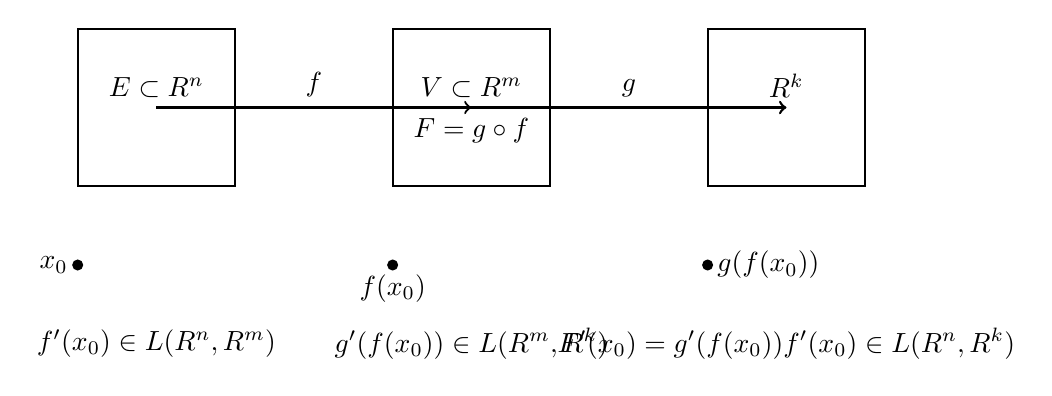
\begin{tikzpicture}
		% Define points
		\coordinate (E) at (0,0);
		\coordinate (V) at (4,0);
		\coordinate (Rk) at (8,0);
		\coordinate (x0) at (0,-1);
		\coordinate (fx0) at (4,-1);
		\coordinate (g_fx0) at (8,-1);

		% Draw sets with square boxes
		\draw[thick] (E) rectangle ++(2,2) node[midway, above] {$E \subset \mathbb{R}^n$};
		\draw[thick] (V) rectangle ++(2,2) node[midway, above] {$V \subset \mathbb{R}^m$};
		\draw[thick] (Rk) rectangle ++(2,2) node[midway, above] {$\mathbb{R}^k$};

		% Draw arrows
		\draw[->, thick] (1,1) -- (5,1) node[midway, above] {$f$};
		\draw[->, thick] (5,1) -- (9,1) node[midway, above] {$g$};
		\draw[->, thick] (1,1) -- (9,1) node[midway, below] {$F = g \circ f$};

		% Draw points and labels
		\fill (x0) circle (2pt) node[left] {$x_0$};
		\fill (fx0) circle (2pt) node[below] {$f(x_0)$};
		\fill (g_fx0) circle (2pt) node[right] {$g(f(x_0))$};

		% Draw derivatives
		\node at (1,-2) {$f'(x_0) \in L(\mathbb{R}^n, \mathbb{R}^m)$};
		\node at (5,-2) {$g'(f(x_0)) \in L(\mathbb{R}^m, \mathbb{R}^k)$};
		\node at (9,-2) {$F'(x_0) = g'(f(x_0)) f'(x_0) \in L(\mathbb{R}^n, \mathbb{R}^k)$};
	\end{tikzpicture}
\end{thm}

\begin{proof}
	\begin{remark}
		Similar to the proof of Theorem~\ref{thm:5.5}.
	\end{remark}
	\begin{flalign*}
		F(x_{0}+h)-F(x_{0}) & =g(f(x_{0}+h))-g(f(x_{0}))=g'(f(x_{0}))+\underbrace{v(k)}_{o(k)}            \\
		                    & =g'(f(x_{0}))\left[f'(x_{0})h+u(h)\right] +v(k)=g'(f(x_{0}))f'(x_{0})h+r(h)
		,\end{flalign*}
	where $r(h)=g'(f(x_{0}))u(h)+v(k)$.\\
	We want to prove that $r(h)=o(h)$; i.e., $\lim_{h\to 0}{\frac{\left|r(h)\right|}{\left|h\right|}}$.
	Note
	\[
		\frac{\left|g'(f(x_{0}))u(h)\right|}{\left|h\right|}  \le \|g'(f(x_{0}))\| \cdot \frac{\left|u(h)\right|}{\left|h\right|}\to 0 \text{ as } h\to 0	\text{ since } u(h)=o(h)
		.\]
	\begin{flalign*}
		\frac{\left|v(k)\right|}{\left|h\right|} & =\frac{\left|v(k)\right|}{\left|k\right|}\cdot \frac{\left|k\right|}{\left|h\right|}\le \frac{\left|v(k)\right|}{\left|k\right|} \left[\frac{\left|f'(x_{0})h\right|}{\left|h\right|}+ \frac{\left|u(h)\right|}{\left|h\right|}\right] \\
		                                         & \le \frac{\left|v(k)\right|}{\left|k\right|} \cdot \left[\|f'(x_{0})\|\cdot \frac{\left|h\right|}{|\left| h \right|}+\frac{\left|u(h)\right|}{\left|h\right|}\right]\to 0 \text{ as } h\to 0
		.\end{flalign*}
	Thus, $r(h)=o(h)$.
\end{proof}
\begin{notation}
	Standard bases of $\R^{n} \text{ and }  \R^{m}$ are denoted by $e_{1},\ldots,e_{n}$ and $u_{1},\ldots,u_{m}$ respectively, where
	\[
		e_{i}=(0,\ldots,0,1,0,\ldots,0),
	\]
	\[
		u_{j}=(0,\ldots,0,1,0,\ldots,0)
		,\]
	where the $1$ is in the $i$-th position.\\
	For $f: \R^{n}\to \R^{m}$, write \[
		f(x)=\sum_{j=1}^{m}{f_j(x) u_j}
		,\] so that
	\[
		f=(f_{1},\ldots,f_{m})
		,\] where $f_j:\R^{n}\to \R$, $f_j(x)= u_j \cdot f$.
\end{notation}

\begin{define}[16][Partial Derivatives]
	For $i=1,2,\ldots n$, $j=1,2,\ldots m$,
	\[
		\frac{\partial f_{i}}{\partial x_{j}}(x)=
		(D_{j}f_{i})(x)=
		\lim_{t\to 0}{\frac{f_{i}(x+te_{j})-f_{i}(x)}{t}} \text{ if the limit exists}
		.\]
\end{define}

\begin{thm}[17]
	If $f:\R^{n}\to \R^{m}$ is differentiable at $x \in \R^{n}$, then
	$(D_i f_j)(x)$ exists for all $i=1,2,\ldots ,n$, $j=1,2,\ldots m$, and
	\[
		\left[f'(x)\right]=\left[\begin{array}{ccc}
				(D_1 f_1)(x) & \ldots & (D_n f_1)(x) \\
				\vdots       &        & \vdots       \\
				(D_1 f_m)(x) & \ldots & (D_n f_m)(x)
			\end{array}\right]
		.\]
	In other words, $\left[f'(x)\right]_{ij}=(D_i f_j)(x)=\frac{\partial f_j}{\partial x_i}(x)$.
\end{thm}
\begin{proof}
	We want to prove that $A=f'(x)$ has matrix elements:
	\[
		u_{i}\cdot A e_{j}=(D_{j}f_{i})(x)=\frac{\partial f_{i}}{\partial x_{j}}(x)
		.\]
	That is, \[
		f_i(+te_j)=f_i(x) + A_{ij}t + o(t)
		.\]
	Let
	\[
		\epsilon(t)=f_i(x+te_j)-f_i(x)-A_{ij}t=u_i \cdot \left[f(x+te_j)-f(x)-A(te_j)\right]
		.\]
	By Cauchy-Schwartz inequality,
	\[
		\left|\epsilon(t)\right|\le \left|u_i\right|\cdot \left|f(x+te_j)-f(x)-A(te_j)\right|
		.\]
	Since $\left|u_i\right|=1$ and
	\[
		\left|f(x+te_j)-f(x)-A(te_j)\right|=o(te_j)=o(t) \;\;(\because \text{ by def. of } f'(x))
		,\]
	we have $\epsilon(t)=o(t)$.
	\begin{note}
		Existence of all partial derivatives does not imply differentiability.
	\end{note}
\end{proof}
\begin{example}
	(see also p.215 of Rudin's)\\
	\begin{enumerate}
		\item
		      (check desmos3d for the graph of)
		      \[
			      f(x,y)=
			      \begin{cases}
				      \frac{xy}{x^2+y^2} & \text{ if } (x,y)\neq (0,0) \\
				      0                  & \text{ if } (x,y)=(0,0)
			      \end{cases}
			      .\]
		      We have
		      \[
			      \frac{\partial f}{\partial x}\bigg{\rvert}_{(0,0)}=\lim_{t\to 0}{\frac{f(t,0)-f(0,0)}{t}}=\lim_{t\to 0}{\frac{0-0}{t}}=0
			      ,\]
		      \[
			      \frac{\partial f}{\partial y}\bigg{\rvert}_{(0,0)}=\lim_{t\to 0}{\frac{f(0,t)-f(0,0)}{t}}=\lim_{t\to 0}{\frac{0-0}{t}}=0
			      .\]
		      However, $f$ is not continuous at $(0,0)$:
		      \[
			      \lim_{t\to 0}{f(t,at)}=\lim_{t\to 0}{\frac{at^2}{t^2+(at)^2}}=\lim_{t\to 0}{\frac{a}{1+a^2}}=\frac{a}{1+a^2}\neq f(0,0) \text{ if } a\neq 0
			      .\]
	\end{enumerate}
\end{example}


\begin{define}[Gradient]
	Let $E \subset \R^{n}$ be open, $f: E\to \R^{1}$.
	If the partial derivatives $\frac{\partial f}{\partial x_{i}}$ exist for all $i=1,2,\ldots n$, then the \textit{gradient} of $f$ at $x \in E$ is given by
	\[
		\nabla f(x)=\sum_{j=1}^{n}{\frac{\partial f}{\partial x_{j}}(x)e_{j}}=
		\left(\frac{\partial f}{\partial x_{1}}(x),\ldots,\frac{\partial f}{\partial x_{n}}(x)\right)
		.\]
	Hence, $\nabla f: E\to \R^{n}$.\\
	If $f'(x)$ exists then the gradient is the matrix representation of $f'(x)$.\\
	In particular, if $h=(h_{1},h_{2},\ldots ,h_n) \in R^{n}$, then \[
		f'(x)h=\nabla f(x) \cdot h=\sum_{i=1}^{n}{\frac{\partial f}{\partial x_{i}}(x)h_{i}}
		.\]
	Also, for $u \in \R^{n}$ with $\left|u\right|=1$,
	\[
		\lim_{t\to 0}{\frac{f(x+tu)-f(x)}{t}}= \frac{\mathrm{d}}{\mathrm{d}t}\bigg{\rvert}_{t=0}{f(x+tu)}=f'(x)u=\nabla f(x) \cdot u
		.\]
	This is the \textit{directional derivative} of $f$ at $x$ in the direction of $u$, and is denoted by $(D_u f)(x)$.
	Note that $(D_u f)(x)=\nabla f(x) \cdot u$ is maximal when $u\parallel \nabla f$.
	Hence, $\nabla f$ points in the direction of maximal increase of $f$ at $x$.
\end{define}
\begin{example}
	Let $z=f(x,y)=x^2+y^2$. Then
	\[
		\nabla f(x,y)=\left(\frac{\partial f}{\partial x},\frac{\partial f}{\partial y}\right)=(2x,2y)
		.\]
	The maximal rate of increase of $f$ at $(x,y)$ is in direction of $\nabla f(x,y)$.
\end{example}

\begin{define}[Convexity]
	A $E \subset \R^{n}$ is \textit{convex} if for all $x,y \in E$ and $\lambda \in [0,1]$, $(1-\lambda) x+\lambda y \in E$.
\end{define}
\begin{example}

\end{example}


\begin{thm}[19]
	Let $E \subset \R^{n}$ be open and convex, and let $f: E\to \R^{m}$.\\
	Suppose $f$ is differentiable on $E$ and $\|f'\|\le M$ for all $x \in E$.
	Then for all $a,b \in E$, we have
	\[
		\left|f(b)-f(a)\right|\le M \left|b-a\right|
		.\]
	\begin{proof}
		Note \[
			f(b)-f(a)=\int_{0}^{1}{\frac{\mathrm{d}}{\mathrm{d}t}f((1-t)a+tb)\mathrm{d}t}
		\]
		by convexity of $E$,  component-wise integration (Theorem 6.23) and Theorem~\ref{thm:ftc}.
		We now have \[
			f(b)-f(a)=\int_{0}^{1}{f'((1-t)a+tb)(b-a)\mathrm{d}t}
			.\]
		Since $f'((1-t)a+tb) \in L(\R^{n},\R^{m})$ and $(b-a) \in \R^{n}$, we have
		\begin{flalign*}
			\left|f(b)-f(a)\right| & = \left|\int_{0}^{1}{f'((1-t)a+tb)(b-a)\mathrm{d}t}\right|                                                                         \\
			                       & \le \int_{0}^{1}{\left|f'((1-t)a+tb)(b-a)\right|\mathrm{d}t}\le \int_{0}^{1}{ M \left|b-a\right|\mathrm{d}t}\le M \left|b-a\right|
			.\end{flalign*}
	\end{proof}
\end{thm}

\begin{corollary}
	\label{cor:9.19}
	If in addition, $f'(x)=0$ all $x \in E$, then $f$ is constant on $E$.
\end{corollary}

\begin{problem}[9.9]
Corollary~\ref{cor:9.19} remains for open connected $E$.
\end{problem}

\begin{define}
	$f:E\to \R^{m}$ is continuously differentiable if $f'(x)$ exists for all $x \in E$ and if $f':E\to L(\R^{n},\R^{m})$ is continuous; i.e., if
	\[
		\forall{x \in E}: \forall{\epsilon > 0}: \exists{\delta > 0} \text{ such that } \left|x-y\right|<\delta, y \in E \implies \|f'(x)-f'(y)\|<\epsilon
		.\]
\end{define}
\begin{notation}
	If $f:E\to \R^{m}$ is continuously differentiable, then we write $f \in \mathcal{C}'(E)$.
\end{notation}

\begin{thm}
	Suppose $f: E\to \R^{m}$, where $E$ is an open subset of $R^{n}.$
	Then $f \in \mathcal{C}'(E) \Leftrightarrow \frac{\partial{f_{i}}}{\partial{x_j}}$ exists for all $i=1,2,\ldots,m$ and $j=1,2,\ldots,n$ and are continuous on $E$.
	\begin{proof}
		check out Rudin's proof.
	\end{proof}

	\begin{note}
		We've seen an example where all $\frac{\partial{f_i}}{\partial{x_j}}$ exist, but $f \not\in \mathcal{C}'(E)$ when the partial derivatives are not continuous.
	\end{note}
\end{thm}
\section{Inverse Function Theorem}
For 1-dimensional case:
(check out Rudin's Problem~5.2)
If $f'(x)>0$ for all $x \in (a,b)$ then $f$ is strictly increasing on $(a,b)$ and thus has an inverse function $g$. This $g$ is differentiable and $g'(f(x))=\frac{1}{f'(x)}$ for all $x \in (a,b)$.

\begin{tikzpicture}[scale=1.2, font=\small]
	% --- LEFT PLOT ---
	% Axes
	\draw[->] (-0.5,0) -- (4.5,0) node[right] {$x$};
	\draw[->] (0,-1.0) -- (0,3.5) node[above] {$y$};

	% Curve y = f(x)
	\draw[thick, smooth, domain=0.5:4] plot (\x, {0.5*(\x-2)^2 + 1}) node[right] {$y = f(x)$};

	% Points on curve
	\coordinate (A) at (2,1);
	\coordinate (B) at (2.8,{0.5*(2.8-2)^2 + 1});

	% Mark points A and B
	\fill (A) circle (1pt) node[below left] {$x$};
	\fill (B) circle (1pt) node[right] {$x + \Delta x$};

	% Draw delta x and delta y arrows
	\draw[->] (A) -- ++(0.8,0) node[midway, below] {$\Delta x$};
	\draw[->] (A) -- (2,{0.5*(2.8-2)^2 + 1}) node[midway, left] {$\Delta y$};

	% Dashed lines to form a triangle
	\draw[dashed] (A) -- (2.8,1);
	\draw[dashed] (2.8,1) -- (B);

	% Tangent line at A
	\draw[dashed, thick] (1.5,0.875) -- (2.5,1.125); % approx tangent

	% Derivative label
	\node at (1.8,2.5) {$g'(f(x)) = \dfrac{1}{f'(x)}$};

	% --- RIGHT PLOT ---
	\begin{scope}[xshift=6cm]

		% Axes
		\draw[->] (-0.5,0) -- (4.5,0) node[right] {$x$};
		\draw[->] (0,-0.5) -- (0,3.5) node[above] {$y$};

		% Curve with a max
		\draw[thick, smooth, domain=0.5:4] plot (\x, {-0.5*(\x-2)^2 + 3}) node[right] {$y = f(x)$};

		% Points with same y-value
		\coordinate (P1) at (1.3, {-0.5*(1.3-2)^2 + 3});
		\coordinate (P2) at (2.7, {-0.5*(2.7-2)^2 + 3});

		% Mark those points
		\draw[dashed] (P1) -- (1.3,0) node[below] {$x_1$};
		\draw[dashed] (P2) -- (2.7,0) node[below] {$x_2$};
		\draw[dashed] (P1) -- (P2);
		\node at (2,2.7) {Inverse does not exist};

	\end{scope}

\end{tikzpicture}

\begin{thm}[24]
	Suppose $f: E\to \R^{n}$, where $E$ is an open subset of $\R^{n}$, is in $\mathcal{C}'(E)$, $a \in E$, $f'(a)$ invertible (c.f., $f'(a)\neq 0$ for $n=1$).
	Let $b = f(a)$. Then
	\begin{enumerate}
		\item there exists an open $U$ containing $a$ and an open $V$ containing $b$ such that $f:U\to V$ is a bijection.
		      [Thus $g=f^{-1}$ exists on $V$ and $g:V\to U$ obeys $g'(f(x))=x$ for all $x \in E$]
		\item $g \in \mathcal{C}'(V)$.
	\end{enumerate}
	\begin{remark}
		\begin{enumerate}
			\item By the chain rule, $g'(f(x))f'(x)=I$; i.e., $g'(f(x))=[f'(x)]^{-1}$ for $x \in U$.
			\item write
			      \begin{flalign*}
				      y_{1} & =f_{1}(x_{1},\ldots,x_{n}) \\
				      y_{2} & =f_{2}(x_{1},\ldots,x_{n}) \\
				            & \vdots                     \\
				      y_{n} & =f_{n}(x_{1},\ldots,x_{n})
				      .\end{flalign*}
			      If $f'(a)$ is invertible, then for $y$ near $b=f(a)$,
			      there exists a unique solution $(x_{1},\ldots,x_{n}) \in C'(E)$ to the system of equations such that
			      \begin{flalign*}
				      x_{1}=g_{1}(y_{1},\ldots,y_{n}) \\
				      x_{2}=g_{2}(y_{1},\ldots,y_{n}) \\
				       & \vdots                       \\
				      x_{n}=g_{n}(y_{1},\ldots,y_{n})
				      .\end{flalign*}
			\item Invertibility of $f'(a)$ is equivalent to the Jacobian determinant of $f$ at $a$ being non-zero; i.e.,
			      \[
				      J_f(a):=
				      \begin{vmatrix}
					      \frac{\partial f_1}{\partial x_1}(a) & \cdots & \frac{\partial f_1}{\partial x_n}(a) \\
					      \vdots                               &        & \vdots                               \\
					      \frac{\partial f_n}{\partial x_1}(a) & \cdots & \frac{\partial f_n}{\partial x_n}(a)
				      \end{vmatrix}
				      \neq 0
				      .\]
		\end{enumerate}
	\end{remark}
\end{thm}

\begin{proof}[Theroem~\ref{thm:9.24}]
	\hfill
	\begin{description}
		\item[Step 1. Existence of open $U$ containing $a$ such that $f$ is one-to-one on $U$:]
		      Write $A=f'(a)$. Given $y \in \R^{n}$, let $\phi:E\to \R^{n}$ by $\phi(x)=x+A^{-1}(y-f(x))$.
		      Then $\phi(x)=x \Leftrightarrow y=f(x)$ [$A^{-1}z=0 \Leftrightarrow z=0$].
		      Therefore, uniqueness of fixed points of $\phi$ would imply uniqueness of $x$ such that $y=f(x)$, which is the one-to-one point of our goal.
		      \begin{note}
			      If $\phi$ is a contraction then fixed points are unique (if there is one) since if $\phi(x_{1})=x_{1}$ and $\phi(x_{2})=x_{2}$, then \[
				      \left|x_{1}-x_{2}\right|=\left|\phi(x_{1})-\phi(x_{2})\right|\le c \left|x_{1}-x_{2}\right|
			      \] with $c<1$ so $x_{1}=x_{2}$.
		      \end{note}
		      Now we have $\phi'(x)=I-A^{-1}f'(x)=A^{-1}(A-f'(x))=A^{-1}(f'(a) - f'(x))$.
		      Hence, \[
			      \|\phi'(x)\|\le \|A^{-1}\|\cdot \underbrace{\|f'(a)-f'(x)\|}_{\le \frac{1}{2 \|A^{-1}\|} \text{ if $\left|x-a\right|<\delta$ for some $\delta>0$ }}
			      .\]
		      Thus, if $x \in N_{\delta}(a)$, then $\|\phi'(x)\|\le \frac{1}{2}$, and $N_\delta(a)$ is the desired open set $U$.
		\item[Step 2. Openness of $V$:]
		      Let $V=f(U)$.
		      Let $y_{0} \in V$, say $y=f(x_{0})$, $x_{0} \in U$.
		      $V$ is then open if and only if for all $y_{0} \in V$, there exists $\epsilon>0$ such that $N_{\epsilon}(y_{0}) \subset V$; i.e., $\forall{y \in N_\epsilon (y_{0})}: \exists{x \in U} \text{ such that } f(x)=y$.\\
		      Given $y \in \R^{n}$, as before, define $\phi_y: E\to \R^{n}$ \[
			      \phi_y(x)=x+A^{-1}(y-f(x))
			      .\]
		      Choose $r>0$ s.t. $\overline{B}=\overline{N_r(x)} \subset U$, which is possible since $U$ is open and $x_{0} \in U$.
		      Next, we show that $\phi_y:\overline{B}\to \overline{B}$ if $y \in N_{\epsilon}(y_{0})$ with $\epsilon$ sufficiently small.
		      In fact, for $x \in \overline{B}$, we have
		      \[
			      \left|\phi_y(x)-x_{0}\right|\le  \left|\phi_y(x)-\phi_y(x_{0})\right|+ \left|\phi_y(x_{0})-x_{0}\right| \le \frac{1}{2}\left|x-x_{0}\right|\le \frac{1}{2}r=\left|A^{-1}(y-f(x_{0}))\right|=\left|A^{-1}(y-y_{0})\right|
			      .\]
		      Hence,
		      \[
			      \left|\phi_y(x_{0})-x_{0}\right|=\left|A^{-1}(y-y_{0})\right|\le \|A^{-1}\| \left|y-y_{0}\right|
			      .\]
		      Choose $\epsilon=\frac{1}{2 \|A^{-1}\|}r$ for $y \in N_{\epsilon}(y_{0})$.
		      Then
		      \[
			      \|A^{-1}\left|y-y_{0}\right|\|\le \|A^{-1}\|\epsilon=\frac{1}{2}r
			      .\]
		      Altogether, we have
		      \[
			      \left|\phi_y(x)-x_{0}\right|\le \frac{1}{2}r+\frac{1}{2}r=r
			      .\]
		      Therefore, \[
			      \phi_y(x) \in \overline{B} \text{ for all } x \in \overline{B} \text{ if } y \in N_{\epsilon}(y_{0})
			      .\]
		      hence, $\phi_y:\overline{B}\to \overline{B}$, and since $\phi_y$ is a contraction and $\overline{B}$ is complete, by Theorem~\ref{thm:9.23}, $\phi_y$ has a unique fixed point $x_{*} \in \overline{B}$, for which $\phi(y)(x_{*})=x_*$.
		      This $x_{*}$ obeys $f(x_{*})=y$, so $y \in V$.
		      Thus, $N_\epsilon(y_{0}) \subset V$.
		      This proves (i). of the theorem.
		\item[$g=f^{-1}:V\to U$ is in $\mathcal{C}^{1}(V)$:]
		      Let $y \in V=f(U)$, $y =f(x), x \in U$.
		      Choose $k$ small enough that $y+k \in V$, say $f(x_K)=y+k$, $x_k \in U$.
		      Let $S=f'(x), T=S^{-1}$.
		      \begin{note}
			      $(f'(x))^{-1}$ exists by Theorem 9.8
			      since $f'(x)$ is close to $f'(a)$ and $f'(a)$ is invertible,
		      \end{note}
		      We want to show $\frac{\left|g(y+k)-g(y)-Tk\right|}{\left|k\right|}\to 0$ as $k\to 0$.
		      We have
		      \begin{flalign*}
			      g(y+k)-g(y)-Tk & = x_k -x - Tk                                             \\
			                     & =- T \left[\underbrace{f(x_k)-f(x)}_{=k}- S(x_k-x)\right]
			      .\end{flalign*}
		      Hence, \[
			      \left|g(y+k)-g(y)-Tk\right|\le  \|T\| \left|f(x_k)-f(x)-S(x_k-x)\right|
			      .\]
		      \begin{claim}
			      \[
				      \frac{1}{\left|k\right|}\le \frac{2 \|A^{-1}\|}{x_k -x}
				      .\]
			      I.e.,
			      \[
				      \left|x_k-x\right|\le  2 \|A^{-1}\| \left|k\right|.
			      \]
		      \end{claim}
		      \begin{proof}
			      $x_k-x=\phi_y(x_k)-\phi_y(x)+A^{-1}k$, so
			      \[
				      \left|x_k-x\right|\le  \left|\phi_y(x_k)-\phi_y(x)\right|+\|A^{-1}\left|k\right|\|\le \frac{1}{2} \left|x_k-x\right|+\|A^{-1}\left|k\right|\| \le 2 \|A^{-1}\| \left|k\right|
				      .\]
		      \end{proof}
		      Since have
		      \[
			      \frac{\left|g(y+k)-g(y)-Tk\right|}{\left|k\right|}\le 2 \|A^{-1}\| \cdot \|T\| \cdot  \frac{\left|f(x_k)-f(x)-S(x_k-x)\right|}{\left|x_k-x\right|}
			      ,\]
		      as $k\to 0$, by the claim, $\left|x_k-x\right|\to 0$, so the right hand side of the inequality goes to $0$ as $k\to 0$ by definition of $S=f'(x)$.
		      This shows that $g'(y)=T$ exists for all $y \in V=f(U)$.
	\end{description}
\end{proof}

